\documentclass[preprint,12pt]{elsarticle}

\usepackage[T1]{fontenc}
\usepackage{newtxtext}
\usepackage{amsmath}
\usepackage{amssymb}
\usepackage{booktabs}
\usepackage{array}
\usepackage{tabularx}
\usepackage{graphicx}
\usepackage{float}
\usepackage{placeins}
\usepackage{xcolor}
\usepackage{tikz}
\usepackage[margin=0.78in]{geometry}
\usepackage{hyperref}
\usepackage[nameinlink,noabbrev]{cleveref}

\graphicspath{{figures/}}
\usetikzlibrary{arrows.meta,positioning,calc,fit,backgrounds}
\setlength{\emergencystretch}{2em}
\setlength{\textfloatsep}{10pt plus 2pt minus 2pt}
\setlength{\floatsep}{8pt plus 2pt minus 2pt}
\hypersetup{
  colorlinks=true,
  linkcolor=blue!70!black,
  citecolor=blue!70!black,
  urlcolor=blue!70!black,
  pdfauthor={},
  pdftitle={Supplementary material for Reinforcement learning with forecast-loss rewards for sensor scheduling under power constraints}
}

\renewcommand{\thesection}{S\arabic{section}}
\renewcommand{\thesubsection}{S\arabic{section}.\arabic{subsection}}
\renewcommand{\thefigure}{S\arabic{figure}}
\renewcommand{\thetable}{S\arabic{table}}
\renewcommand{\theequation}{S\arabic{equation}}

\begin{document}

\begin{frontmatter}
\title{Supplementary material for\\
Reinforcement learning with forecast-loss rewards for sensor scheduling under power constraints}
\end{frontmatter}

This document provides implementation details for the Prediction-Driven
Proximal Policy Optimization (PD-PPO) scheduler, baseline definitions,
additional protocol diagnostics, and the 24-seed descriptive aggregate
referenced by the anonymous manuscript. It introduces no additional training
or model selection.

\section*{Terminology guide}

The following terms are used consistently in the manuscript and this
supplement.

\begingroup
\footnotesize
\setlength{\tabcolsep}{4pt}
\renewcommand{\arraystretch}{1.08}
\noindent\begin{tabularx}{0.96\linewidth}{@{}>{\raggedright\arraybackslash}p{0.27\linewidth}>{\raggedright\arraybackslash}X@{}}
  \toprule
  Term & Meaning in this study \\
  \midrule
  PD-PPO scheduler & Complete scheduler comprising input construction, the policy, feasibility check, and execution constraint. \\
  Primary forecaster & Temporal convolutional network (TCN) trained on the forecaster-training partition. \\
  Frozen primary forecaster & Primary forecaster after its parameters are fixed for policy training and offline evaluation. \\
  Policy & Parameterized masked distribution $\pi_\theta$ over feasible proposed action indices. \\
  Meteorological core channel & Mandatory logical channel active in every channel subset. \\
  Optional channel & Any of the other five logical channels. \\
  Other optional channels & Basic radiometer channel and shielded temperature--humidity channel. \\
  Specialist channels & Infrared snow-surface-temperature channel, laser disdrometer channel, and FC4 snow mass-flux channel. \\
  Channel subset & Set of requested logical channels at one time step. \\
  Activation vector & Binary mathematical representation of a channel subset. \\
  Proposed action index $u_t$ & Categorical policy selection identifying one proposed candidate channel subset. \\
  Feasible-action mask & Indicator over candidate actions after the feasibility check. \\
  Minimum dwell-time constraint & Keeps the previously executed channel subset active until its minimum dwell time is met. \\
  Sample-and-hold value & Last valid measurement retained when no new measurement is available. \\
  Observation mask & Indicator that a variable received a new observation at the current time step. \\
  Current condition label $c_t$ & Simulator-derived current operating-condition label used for training-loss weighting and offline evaluation, not as a deployed policy input. \\
  Future-condition supervision label $c_t^{\mathrm{sup}}$ & First non-calm label from $t$ through $t+16$, or calm if none occurs; used only for policy-training supervision. \\
  Channel sampling age & Time since the channel's last ready sampling opportunity; distinct from variable-level age of information (AoI). \\
  Validation-selected fixed-schedule baseline & Fixed channel subset selected on the calibration/validation partition. \\
  AoI-priority baseline & Feasible dynamic baseline prioritizing age of information. \\
  Round-robin baseline & Baseline that uses a fixed cyclic schedule over candidate channel subsets. \\
  Random-feasible baseline & Baseline sampled from the feasible action set. \\
  Privileged one-step look-ahead reference using next-step test targets & Reference that selects the feasible action with the lowest next-step forecast loss on the test partition while omitting longer dynamic consequences from its objective. \\
  Warning-rule baseline & Deterministic baseline driven by simulated warning signals. \\
  Privileged true-label baseline & Baseline using the exact label sequence $c_t,\ldots,c_{t+16}$ at each decision. \\
  Double DQN training configuration & Training-configuration comparison using the same state representation, reward, action set, and constraints; it omits behavior cloning pretraining, continuing advantage-weighted behavior cloning, and the auxiliary future-condition classifier used by the complete PD-PPO configuration. \\
  Macro-averaged normalized forecast loss & Equal-weight mean of the three event-type-specific losses after calibration/validation-based normalization. \\
  \bottomrule
\end{tabularx}
\endgroup


\section{Recent-history features and policy encoding}

The scheduler input contains ten deterministic recent-history features. Let
\(\bar{x}_{t,j}\) be the sample-and-hold value normalized by
forecaster training statistics and clipped to \([-5,5]\), let
\(\Delta_{16}\bar{x}_{t,j}=\bar{x}_{t,j}-\bar{x}_{t-15,j}\), and let
\(C_{16}(\mathcal{J})\) be the largest 16-step observation fraction among
variables in \(\mathcal{J}\). Three event-related recent-history features are
\begin{align}
 b_t^{\mathrm{part}} &=
 \tanh(0.45\bar v_{p,t}+0.25\bar d_{p,t}+0.15\bar f_t),\\
 b_t^{\mathrm{flux}} &=
 \tanh(0.55\bar f_t+0.25\bar v_{\mathrm{wind},t}+0.10\Delta_{16}\bar f_t),\\
 b_t^{\mathrm{therm}} &=
 \tanh\!\left(0.45(\bar T_{a,t}-\bar T_{s,t})
 -0.10\Delta_{16}\bar T_{s,t}\right).
\end{align}
Here \(v_{\mathrm{wind}}\), \(f\), \(v_p\), \(d_p\), \(T_a\), and \(T_s\) denote wind
speed, snow mass flux, particle velocity, particle diameter, air temperature,
and snow-surface temperature. The three indicators are concatenated with current
normalized wind speed, snow mass flux, particle velocity, the air--surface
temperature difference, and the particle, flux, and thermal coverage terms.
Every component is computed from sample-and-hold values and observation masks;
this information is available at decision time.

The policy uses the aggregate warning signal \(q_t^{\max}\) to combine two observation-history
encoders,
\begin{equation}
  h_t=(1-g_t)f_0(o_t)+g_t f_1(o_t),\qquad
  g_t=\operatorname{sigmoid}(\alpha q_t^{\max}+\beta),
\end{equation}
where \(\alpha\), \(\beta\), and both encoders are learned. A candidate
activation vector \(a^{(u)}\) is represented by the sum of learned embeddings of
its active channels. Its policy score is the scaled inner product between the
subset embedding and \(h_t\), plus a learned subset bias. The
feasible-action mask excludes infeasible action indices before categorical sampling. The critic receives \(o_t\) and
\(q_t^{\max}\) through a separate multilayer perceptron.

\section{Forecaster and policy training protocol}

The primary forecaster is fitted on 78 rollouts containing 53,274 time steps,
all drawn from the forecaster-training partition. Its parameters are then frozen
during policy training and evaluation. The full-observation baseline contributes
18 rollouts. A feasible fixed-schedule source and the round-robin, AoI-priority,
and random-feasible baselines contribute six each, as does each of the six fixed
channel subsets. Each rollout contains 683 time steps. For each schedule, three
starts are event centered and three are sampled uniformly from the
forecaster-training partition. At reset, all channels are off, the 20-step
observation history is initialized to the
mean of that partition, and its observation masks are zero. No
calibration/validation or test observation enters the training mixture.

\begin{table}[htbp]
  \centering
  \caption{Main protocol and PD-PPO scheduler hyperparameters for the reported experiment.}
  \label{tab:main_protocol_hyperparameters}
  \scriptsize
  \renewcommand{\arraystretch}{0.82}
  \setlength{\tabcolsep}{3.2pt}
  \begin{tabular}{@{}p{0.38\linewidth}p{0.55\linewidth}@{}}
    \toprule
    Item & Value \\
    \midrule
    Reported seeds & 117--140: pilot/model-selection seeds 117--118; post-selection evaluation seeds 119--140 \\
    Simulated series length & 70,000 hourly time steps per seed \\
    Chronological partitions & [0,24500) forecaster training; [24500,59500) policy training; [59500,64750) calibration/validation (normalization-factor computation and fixed-baseline selection); [64750,70000) test \\
    Forecast lookback / horizon & 20 / 8 time steps; uniform horizon weights \\
    Event-balanced test windows & 8 windows selected from test truth to balance event types and emphasize transport periods, 512 time steps each; selection uses no policy losses \\
    Full test-partition evaluation & All 5,242 scoreable test time steps; same trained policies, channel subsets, and normalization factors \\
    Candidate action set & 6 candidate channel subsets \\
    Mandatory channel & Meteorological core channel \\
    Steady-state / startup-peak power limits & 0.75 / 0.95 \\
    Constraint activation in the reported candidate set & Maximum steady/startup demand 0.74/0.92; all six candidates feasible at every step; optional-channel cardinality and minimum dwell time are the active restrictions \\
    Policy timesteps & 200,000 \\
    PPO rollout / batch / update epochs & 1024 / 128 / 8 \\
    Recent-history features & 16-step normalized values, slopes, and observation coverage; 10 features \\
    Policy/critic network & two 128-unit feature encoders combined by the aggregate warning signal; 32-dimensional embeddings of candidate channel subsets; separate warning-aware critic \\
    Learning rate, discount, GAE & 0.0003, 0.99, 0.95 \\
    Clip, entropy, value coef. & 0.2, 0.0075, 0.5 \\
    Continuing advantage-weighted behavior cloning and auxiliary future-condition classifier weights & $\beta_{\mathrm{BC}}=2.5$; $\beta_{\mathrm{cond}}=5.0$ \\
    Condition-specific training weights & particle/flux/thermal = 1.55/0.95/1.65; calm = 1.0 \\
    Calibration/validation-based normalization factors & event-type-specific median over fixed channel subsets for particle/flux/thermal; default overall-loss median for calm \\
    Future-condition supervision label & first non-calm condition label from $t$ through $t+16$, or calm if none occurs; training only \\
    Minimum dwell time / normalized switching-cost weight / warm-up interruption-cost weight & 6 time steps; 0.001; 1.0 \\
    Fixed-baseline selection metric & macro-averaged normalized forecast loss \\
    Event-type mix & particle/flux/thermal = 0.40/0.20/0.40 \\
    Event coverage target & 0.68 \\
    Statistical resampling & 100,000 percentile-bootstrap samples over paired seed differences; seed 20,260,718 \\
    Behavior cloning pretraining & 10,000 steps; 18 epochs; batch size 256 \\
    \bottomrule
  \end{tabular}
  \vspace{0.2ex}

  \noindent\scriptsize
  Partitions are fixed before test evaluation; fixed-baseline selection and
  normalization factors use only the calibration/validation partition.
\end{table}

\begin{table}[htbp]
  \centering
  \caption{Scalar-objective PPO configurations, Double DQN training configuration, and primary-forecaster
  training protocol.}
  \label{tab:control_protocol_hyperparameters}
  \scriptsize
  \renewcommand{\arraystretch}{0.86}
  \setlength{\tabcolsep}{3.2pt}
  \begin{tabular}{@{}p{0.38\linewidth}p{0.55\linewidth}@{}}
    \toprule
    Item & Value \\
    \midrule
    Scalar-objective PPO variants & Same PPO policy and critic architecture, scheduler input, action set, constraints, behavior cloning pretraining, continuing advantage-weighted behavior cloning, and auxiliary future-condition classifier; replace forecast loss with normalized target AoI or a bounded diagonal uncertainty proxy \\
    Double DQN training configuration & Dueling 128-unit network; 200,000 steps; experience replay 100,000; learning starts 5,000; batch 128; 3-step return; target update 1,000; $\epsilon$ 1.0 to 0.05 over 20\%; learning rate $10^{-4}$; no behavior cloning pretraining, continuing advantage-weighted behavior cloning term, or auxiliary future-condition classifier \\
    Primary forecaster architecture & residual TCN, 3 levels, 64 channels, kernel size 3, dropout 0.05 \\
    Forecaster-training mixture & 78 rollouts (53,274 time steps). The mixture contains 18 full-observation rollouts, six for each dynamic baseline or feasible fixed-schedule source, and six for each fixed channel subset. \\
    Normalization & forecaster input/target scales fitted before policy updates; calibration/validation-based normalization factors computed before policy optimization \\
    Checkpoint/baseline handling & final policy checkpoint saved after the prescribed PPO updates; fixed baseline selected by lowest calibration/validation macro-averaged loss \\
    Computation & GPU policy optimization; the same frozen primary forecaster for all test metrics \\
    \bottomrule
  \end{tabular}
\end{table}


Each event-balanced test window is evaluated as a separate rollout. At its
start, all channel runtimes are off, the previous activation vector and
remaining required activation time are zero, the sample-and-hold values and 20-step history are
initialized to the configured state mean, and observation masks are zero. The
policy or minimum dwell-time wrapper state is also reset.
No pre-roll context is supplied. Metrics concatenate the eight 512-step
rollouts; action-transition diagnostics therefore include the seven boundaries
between separately reset windows. Continuous full-partition evaluation instead
uses one reset at time step 64,750 followed by one 5,242-step rollout.

\begin{figure}[htbp]
  \centering
  \resizebox{\linewidth}{!}{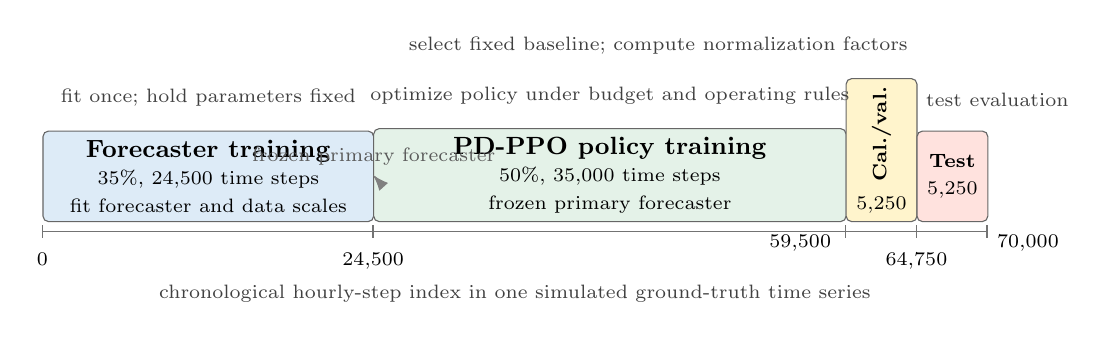
\begin{tikzpicture}[
  font=\small,
  axis/.style={line width=0.6pt, draw=black!55},
  splitbox/.style={
    draw=black!60,
    rounded corners=2pt,
    minimum height=1.15cm,
    align=center,
    inner xsep=3pt,
    inner ysep=3pt
  },
  note/.style={font=\scriptsize, align=center, text=black!75},
  flow/.style={-{Latex[length=2mm]}, line width=0.55pt, draw=black!50}
]

\definecolor{forecasterblue}{RGB}{221,235,247}
\definecolor{rlgreen}{RGB}{228,242,232}
\definecolor{valyellow}{RGB}{255,244,204}
\definecolor{testred}{RGB}{255,226,222}

% The x coordinates encode the 35/50/7.5/7.5 chronological split.
\coordinate (x0) at (0,0);
\coordinate (x1) at (4.20,0);
\coordinate (x2) at (10.20,0);
\coordinate (x3) at (11.10,0);
\coordinate (x4) at (12.00,0);

\node[splitbox, fill=forecasterblue, minimum width=4.20cm, anchor=south west]
  (forecasterfit) at (x0)
  {\textbf{Forecaster training}\\[-1pt]\scriptsize 35\%, 24{,}500 time steps\\[-1pt]\scriptsize fit forecaster and data scales};
\node[splitbox, fill=rlgreen, minimum width=6.00cm, anchor=south west]
  (rltrain) at (x1)
  {\textbf{PD-PPO policy training}\\[-1pt]\scriptsize 50\%, 35{,}000 time steps\\[-1pt]\scriptsize frozen primary forecaster};
\node[splitbox, fill=valyellow, minimum width=0.90cm, anchor=south west]
  (val) at (x2)
  {\rotatebox{90}{\scriptsize\textbf{Cal./val.}}\\[-1pt]\scriptsize 5{,}250};
\node[splitbox, fill=testred, minimum width=0.90cm, anchor=south west]
  (test) at (x3)
  {\scriptsize\textbf{Test}\\[-1pt]\scriptsize 5{,}250};

% Short process notes above the timeline. These are intentionally terse to avoid
% crowding the narrow validation/test blocks.
\node[note, above=0.18cm of forecasterfit] {fit once; hold parameters fixed};
\node[note, above=0.18cm of rltrain] {optimize policy under budget and operating rules};
\node[note, anchor=south east] at ([yshift=0.18cm]val.north east)
  {select fixed baseline; compute normalization factors};
\node[note, anchor=south west] at ([yshift=0.18cm]test.north west)
  {test evaluation};

\draw[flow, dashed] (forecasterfit.east) -- node[above, font=\scriptsize, text=black!65]
  {frozen primary forecaster} (rltrain.west);

\draw[axis] (0,-0.12) -- (12.00,-0.12);
\foreach \x in {0,4.20,10.20,11.10,12.00} {
  \draw[axis] (\x,-0.20) -- (\x,-0.04);
}
\node[font=\scriptsize, below=2pt] at (0,-0.20) {$0$};
\node[font=\scriptsize, below=2pt] at (4.20,-0.20) {$24{,}500$};
\node[font=\scriptsize, below=2pt, anchor=east] at (10.14,-0.20) {$59{,}500$};
\node[font=\scriptsize, below=2pt] at (11.10,-0.20) {$64{,}750$};
\node[font=\scriptsize, below=2pt, anchor=west] at (12.00,-0.20) {$70{,}000$};

\node[font=\scriptsize, text=black!75, below=0.55cm] at (6.00,-0.12)
  {chronological hourly-step index in one simulated ground-truth time series};

\end{tikzpicture}
}
  \caption{Chronological data partitions used in the experiments. Forecaster training,
  policy training, calibration/validation, and testing occupy separate intervals.
  The calibration/validation partition is used to select the fixed baseline and
  compute normalization factors and the supervised-action mapping before policy optimization;
  the test partition supplies the event-balanced test windows and evaluation over all
  scoreable test time steps. The two pilot/model-selection seeds use selected
  test-window metrics for the prespecified architecture comparison; the other 22
  seeds are evaluated after that configuration is fixed.}
\end{figure}

\FloatBarrier
\section{Matched scalar-objective PPO configurations}

For the configured observed-variable set $\mathcal{J}$ and history length $H$,
the AoI-objective PPO configuration
uses
\begin{equation}
  \mathcal{L}_{\mathrm{AoI}}(t)
  =\frac{1}{|\mathcal{J}|}\sum_{j\in\mathcal{J}}
  \min\left(\frac{A^{\mathrm{var}}_{t,j}}{H-1},1\right),
\end{equation}
where $A^{\mathrm{var}}_{t,j}$ is the variable-level AoI, measured in time steps
since the latest valid observation of
variable $j$ in the input history. A variable with no valid observation in the
history receives unit loss.

The uncertainty-objective PPO configuration maintains a bounded diagonal predict--update
variance proxy only for its reward. For
each variable, it applies
\begin{equation}
  P^-_{t,j}=\min(P_{t-1,j}+Q_j,P_{\max}),\qquad
  P_{t,j}=\left[(P^-_{t,j})^{-1}+R_{t,j}^{-1}\right]^{-1}
\end{equation}
when a valid observation is available, and $P_{t,j}=P^-_{t,j}$ otherwise.
$R_{t,j}$ is the inverse-variance fused measurement variance. Its bounded
reward proxy is
\begin{equation}
  \mathcal{L}_{\mathrm{unc}}(t)
  =\frac{1}{|\mathcal{J}|}\sum_{j\in\mathcal{J}}
  \frac{P_{t,j}}{1+P_{t,j}} .
\end{equation}
Both scalar-objective PPO variants retain the same condition-specific training
weights, behavior cloning pretraining, continuing advantage-weighted behavior
cloning loss, and auxiliary future-condition classification loss
as PD-PPO. The current operating-condition label $c_t$ supplies the training
weight. The future-condition supervision label $c_t^{\mathrm{sup}}$ is the first
non-calm label from $t$ through $t+16$, or calm if no event occurs in that window;
it supplies the supervised target action and auxiliary future-condition classification
target. Under the reported stride-one configuration both labeled-example
indicators are one at every PPO step, so $\eta_t=\ell_t$; the general
implementation constructs them separately.
Neither label is available to the policy or critic at decision time. The diagonal uncertainty
proxy is distinct from the general estimator covariance trace analyzed in
Proposition 2 of the main manuscript.

\section{Physical platform motivation}

\begin{figure}[htbp]
  \centering
  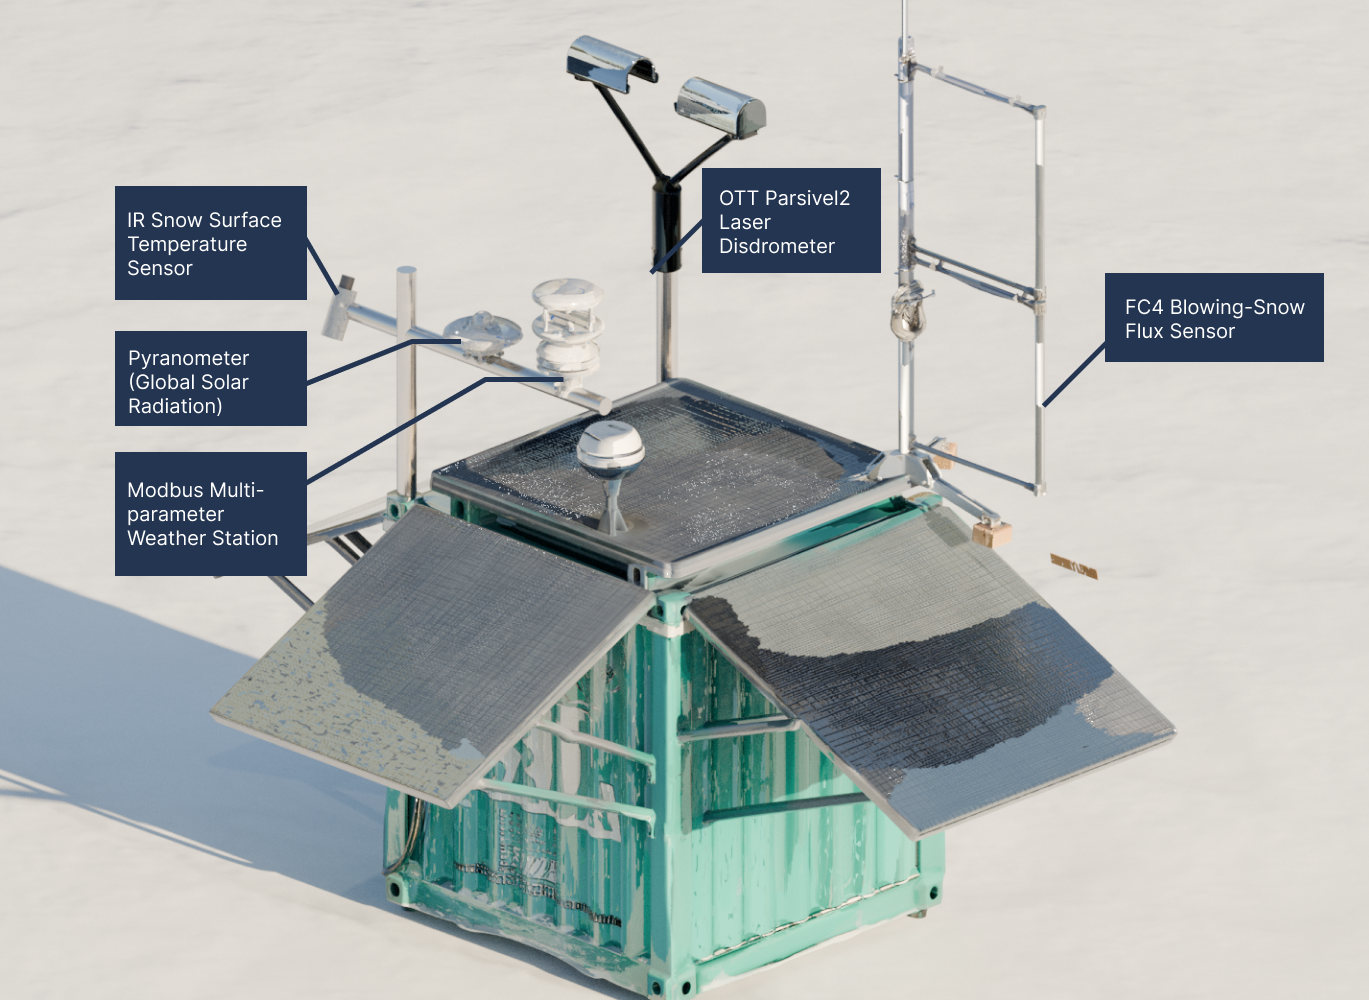
\includegraphics[width=0.78\linewidth]{aws_deployment.png}
  \caption{Rendered automatic weather station platform motivating the reported
  sensing abstraction. The logical channel table in the main manuscript defines
  the experimental sensing system.}
\end{figure}

\FloatBarrier
\section{Simulation model and observation specification}

The meteorological background series is generated by phase-randomizing contiguous
reference time series from Antarctic AWS stations and matching the empirical
marginal distribution of each variable. An alternating calm/storm semi-Markov
process supplies longer calm and storm intervals. Their durations are sampled from a lognormal
distribution, after which event pulses with bounded duration and gap are placed
inside storm intervals. Wind credibility and hysteresis convert candidate
pulses into event intervals. One of the particle, flux, or thermal event
types is sampled for each complete event run.

Within an event run, each event-type process follows a first-order
low-pass process
\begin{equation}
  z_{t,c}=(1-\alpha)z_{t-1,c}+\alpha\epsilon_{t,c},
  \qquad \epsilon_{t,c}\sim\mathcal{N}(0,1),
\end{equation}
and is standardized over its active interval. Event-type effects enter the
target variables after a six-time-step lag. Table S3 lists the simulation-model parameters used
in the reported experiment.

\begin{table}[htbp]
  \centering
  \caption{Parameters of the simulation model. One time step
  equals one hour.}
  \label{tab:simulator_event_parameters}
  \scriptsize
  \renewcommand{\arraystretch}{0.92}
  \setlength{\tabcolsep}{3pt}
  \begin{tabular}{@{}p{0.35\linewidth}p{0.20\linewidth}p{0.38\linewidth}@{}}
    \toprule
    Component & Value & Role \\
    \midrule
    Reference distributions from Antarctic AWS stations
      & Panda100, Panda200, Taishan
      & Phase-randomized Antarctic AWS series with empirical marginal matching. \\
    Sequence length and interval
      & 70,000; 1 h
      & One independently generated simulated ground-truth time series per seed. \\
    Simulated blowing-snow event process
      & alternating semi-Markov storm/calm phases
      & Lognormal phase duration with log-scale standard deviation 0.35 and a
        minimum duration of 24 time steps. \\
    Storm / within-storm event duty
      & 0.65 / 0.78
      & Derived from the event-coverage target after clipping. \\
    Median storm / calm duration
      & 1,440 / 775 time steps
      & Parameters of the alternating calm/storm process. \\
    Event pulse duration / gap
      & Uniform 28--80 / 8--10 time steps
      & Bursty blowing-snow episodes within storm phases. \\
    Wind thresholds and event margin
      & 8 / 12 / 1.4 m s$^{-1}$
      & Weak threshold, strong threshold, and event wind-floor margin. \\
    Hysteresis on / off
      & 0.60 / 0.30
      & Converts candidate pulses and wind credibility into event intervals. \\
    Particle / flux / thermal probability
      & 0.40 / 0.20 / 0.40
      & One event type is sampled for each complete event run. \\
    Event-type process smoothing
      & 0.65
      & Low-pass coefficient for event-type-specific simulated processes. \\
    Target-effect lag
      & 6 time steps
      & Delay from the event-type process to target effects. \\
    Particle process scales
      & 0.62 mm; 8.2 m s$^{-1}$
      & Diameter and particle-velocity effects. \\
    Flux process map
      & scale 0.0014; offset 1.25; clip 2.4
      & Linear event-type effect before clipping. \\
    Thermal process scale
      & 6.4 $^{\circ}$C
      & Snow-surface-temperature effect. \\
    Warning-signal lead / noise
      & 16 time steps / 0.01
      & Linear pre-event ramp plus Gaussian noise, clipped to $[0,1]$. \\
    \bottomrule
  \end{tabular}
\end{table}


Table S4 records the target scales and task weights used by the primary and ridge
forecasters. The current operating-condition label $c_t$ selects a predeclared weight vector after an
observation sequence has been produced by a schedule; it never changes the
scheduler input.

\begin{table}[H]
  \centering
  \caption{Target scales and event-type-dependent weights used with the primary
  forecaster. Zero-weight variables remain forecaster inputs but
  do not enter the reported loss.}
  \label{tab:forecast_target_weights}
  \scriptsize
  \setlength{\tabcolsep}{3.0pt}
  \begin{tabular}{@{}lccccc@{}}
    \toprule
    Forecast target & Scale & Calm/default & Particle & Flux & Thermal \\
    \midrule
    Air temperature & 5 & 0.10 & 0 & 0 & 0.22 \\
    Snow-surface temperature & 5 & 0.26 & 0 & 0 & 85 \\
    Wind speed & 5 & 0.08 & 0.08 & 0.04 & 0.08 \\
    Wind direction sine & 1 & 0 & 0 & 0 & 0 \\
    Wind direction cosine & 1 & 0 & 0 & 0 & 0 \\
    Solar radiation & 100 & 0 & 0 & 0 & 0 \\
    Snow mass flux & $10^{-4}$ & 4.5 & 0.5 & 7 & 0.2 \\
    Particle diameter & 0.2 & 42 & 105 & 5 & 1 \\
    Particle velocity & 5 & 42 & 105 & 5 & 1 \\
    \bottomrule
  \end{tabular}
\end{table}


For each event type $c$, the simulated warning signal is
\begin{equation}
  q_{t,c}=\operatorname{clip}_{[0,1]}
  \left(b_{t,c}+\varepsilon_{t,c}\right),
\end{equation}
where $b_{t,c}=1$ during the event interval, increases linearly during the 16
time steps before onset, and is zero otherwise; $\varepsilon_{t,c}$ is Gaussian
noise with standard deviation 0.01. The aggregate warning signal is
$\max_c q_{t,c}$. The PD-PPO scheduler receives these four simulated warning
signals but neither $c_t$ nor $c_t^{\mathrm{sup}}$. This is a simulation assumption
and has not been validated as a field detector.

An active and ready channel observes variable $j$ with configured probability
$p_{i,j,c}$ and adds independent Gaussian noise with standard deviation
$\sigma_{i,j,c}$. Table S5 gives the event-dependent values of the three
specialist channels. The meteorological core channel uses standard deviations
0.18 m s$^{-1}$ for wind speed, 1.8
degrees for wind direction, 0.18 $^{\circ}$C for air temperature, 0.90
percentage points for relative humidity, and 14 Pa for pressure. The radiometer
uses 8 W m$^{-2}$, while the shielded temperature--humidity channel uses 0.06 $^{\circ}$C
and 0.30 percentage points.

\begin{table}[htbp]
  \centering
  \caption{Availability probabilities and Gaussian noise standard deviations for
  the three specialist logical channels. Entries within a cell follow the variable order
  shown in the second column. ``Other event'' means an active non-matching
  event type.}
  \label{tab:specialist_observation_model}
  \scriptsize
  \renewcommand{\arraystretch}{0.92}
  \setlength{\tabcolsep}{2.7pt}
  \begin{tabular}{@{}p{0.17\linewidth}p{0.25\linewidth}p{0.16\linewidth}p{0.16\linewidth}p{0.18\linewidth}@{}}
    \toprule
    Specialist logical channel & Variables & Calm $(p,\sigma)$ & Other event $(p,\sigma)$ & Matching event type $(p,\sigma)$ \\
    \midrule
    Infrared snow-surface-temperature channel
      & snow-surface temperature; thermal process
      & (0.20, 1.40); (0.10, 1.20)
      & (0.25, 1.60); (0.18, 1.20)
      & (0.96, 0.07); (0.98, 0.03) \\
    Laser disdrometer channel
      & diameter; particle velocity; particle process
      & (0.10, 1.20); (0.10, 3.00); (0.05, 1.50)
      & (0.18, 0.90); (0.18, 2.80); (0.12, 1.20)
      & (0.96, 0.06); (0.96, 0.16); (0.98, 0.03) \\
    FC4 snow mass-flux channel
      & snow mass flux; flux process
      & (0.10, $5.0\!\times\!10^{-6}$); (0.05, 1.50)
      & (0.18, $4.0\!\times\!10^{-6}$); (0.12, 1.20)
      & (0.96, $2.5\!\times\!10^{-7}$); (0.98, 0.03) \\
    \bottomrule
  \end{tabular}
  \vspace{0.4ex}

  \noindent\scriptsize
  Noise is expressed in the physical units of each variable. The process
  variables are simulation-model constructs used to make event-dependent channel
  value explicit; they are distinct from the condition labels.
\end{table}


\FloatBarrier
\section{Executable baseline definitions}

The fixed channel subset selected on the calibration/validation partition is
\begin{equation}
  a_{\mathrm{fixed}}
  =\arg\min_{a\in\mathcal{A}}
  \left(L_{\mathrm{macro,val}}(a),
        L_{\mathrm{val}}(a),
        \operatorname{index}(a)\right),
\end{equation}
with lexicographic ordering. This fixed channel subset is selected before test
evaluation. The warning-rule baseline uses the same calibration/validation procedure
separately for calm, particle, flux, and thermal windows. At time step $t$, it chooses
\begin{equation}
  \widehat{c}_t=
  \begin{cases}
    \arg\max_c q_{t,c}, & \max_c q_{t,c}\geq 0.5,\\
    \mathrm{calm}, & \text{otherwise},
  \end{cases}
\end{equation}
and requests the channel subset selected on the calibration/validation partition
for $\widehat{c}_t$.

The privileged one-step look-ahead reference using next-step test targets
snapshots the complete environment, executes each candidate once, restores the
snapshot, and minimizes
\begin{equation}
  \left(
  L_{\mathrm{step}}(t;a),
  \frac{1}{N}\lVert a-a_{t-1}\rVert_1,
  \operatorname{index}(a)
  \right).
\end{equation}
It uses next-step test targets that are unavailable to the deployed scheduler.
The privileged true-label baseline receives the exact label sequence
$c_t,\ldots,c_{t+16}$ at each decision; this sequence is also unavailable to the
deployed scheduler and differs from the single derived supervision label
$c_t^{\mathrm{sup}}$. Table S6 states all baseline procedures and their information
availability.

\begin{table}[H]
  \centering
  \caption{Definitions of the baselines. All constrained baselines use the same
  candidate action set, feasibility check, channel warm-up model, and six-time-step
  minimum dwell-time constraint as PD-PPO unless
  stated otherwise.}
  \label{tab:executable_baseline_definitions}
  \scriptsize
  \renewcommand{\arraystretch}{0.92}
  \setlength{\tabcolsep}{2.6pt}
  \begin{tabular}{@{}p{0.19\linewidth}p{0.31\linewidth}p{0.25\linewidth}p{0.19\linewidth}@{}}
    \toprule
    Baseline & Decision rule & Selection and tie break & Information availability \\
    \midrule
    Fixed-schedule baseline
      & Apply one fixed channel subset.
      & Evaluate all six subsets on calibration/validation windows; minimize the
        macro-averaged normalized forecast loss, then mean forecast loss.
      & Feasible baseline; no condition labels at decision time. \\
    Fixed-priority baseline
      & Assign linearly decreasing scores by channel index at every time step.
      & Deterministic projector order.
      & Online and non-learned. \\
    Round-robin baseline
      & Give the highest scores to a cyclic group of two channels.
      & The time step and channel index define a fixed cyclic schedule; projection resolves conflicts.
      & Online and non-learned. \\
    AoI-priority baseline
      & Score each channel by clipped time since its last ready sampling opportunity.
      & Project the descending score order.
      & Online and non-learned. \\
    Random-feasible baseline
      & Draw independent Gaussian channel scores at each time step.
      & One random stream per simulation seed, seeded by simulation seed plus 100; the same 512-score stream restarts at each event-balanced test-window reset; project the sampled ranking.
      & Online stochastic baseline; no within-seed Monte Carlo averaging. \\
    Double DQN training configuration
      & Evaluate six Q-values and greedily select the largest currently feasible
        action during test evaluation.
      & Double DQN target with a feasible-action mask; deterministic
        lowest-index tie break.
      & Online learned baseline; no condition labels at decision time. \\
    Warning-rule baseline
      & Choose the largest particle, flux, or thermal warning signal when it is
        at least 0.5; otherwise choose the calm action.
      & On calibration/validation windows, separately minimize calm or event-type loss for
        each warning-signal case; break ties by mean forecast loss.
      & Uses simulated warning signals; no condition labels at decision time. \\
    Privileged one-step look-ahead reference using next-step test targets
      & Simulate every candidate for one time step and select the smallest next-step
        forecast loss on the test partition under the frozen primary forecaster.
      & Lower switching fraction, then lower action index.
      & Uses next-step test targets unavailable to the deployed scheduler; the objective omits minimum dwell-time, warm-up, and observation-age consequences. \\
    Privileged true-label baseline
      & Choose the optional channel selected on the calibration/validation partition using the exact
        label sequence $c_t,\ldots,c_{t+16}$.
      & Use the first active event type in the future-label interval; break calibration/validation
        ties by mean forecast loss.
      & Uses condition labels unavailable to the deployed scheduler. \\
    Full-observation baseline
      & Request all six channels at every time step.
      & No selection.
      & Deliberately removes the constraints; unconstrained benchmark. \\
    \bottomrule
  \end{tabular}
\end{table}


\FloatBarrier
\section{Simulation validation and additional results}

\begin{figure}[htbp]
  \centering
  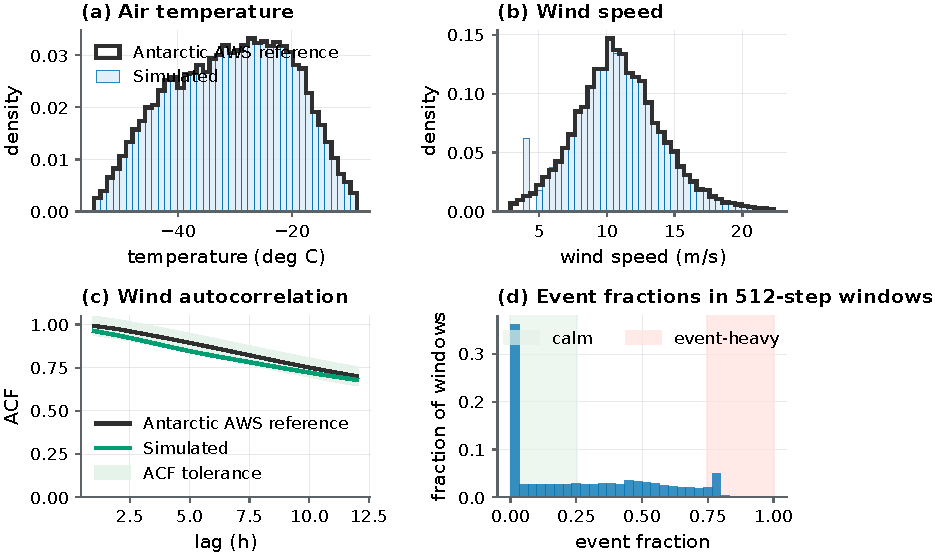
\includegraphics[width=\linewidth]{figure3_synthetic_statistics.pdf}
  \caption{Simulation-validation diagnostics covering agreement between
  simulated and Antarctic-reference distributions, the wind-speed
  autocorrelation function (ACF), and event fractions.}
\end{figure}

\begin{table*}[htbp]
  \centering
  \caption{Sensitivity to evaluation coverage in the test partition. A positive paired difference means that the fixed-schedule baseline has higher loss than PD-PPO.}
  \label{tab:clean_full_partition_sensitivity}
  \scriptsize
  \renewcommand{\arraystretch}{1.05}
  \setlength{\tabcolsep}{2.2pt}
  \begin{tabular}{@{}>{\raggedright\arraybackslash}p{0.16\textwidth}>{\centering\arraybackslash}p{0.06\textwidth}>{\centering\arraybackslash}p{0.13\textwidth}>{\raggedright\arraybackslash}p{0.17\textwidth}>{\centering\arraybackslash}p{0.13\textwidth}>{\raggedright\arraybackslash}p{0.17\textwidth}@{}}
    \toprule
    Evaluation scope & Time steps per seed & Mean forecast loss\newline (PD-PPO / fixed baseline) & Seeds with lower loss;\newline mean paired difference\newline [95\% bootstrap CI] & Macro-averaged loss\newline (PD-PPO / fixed baseline) & Seeds with lower loss;\newline mean paired difference\newline [95\% bootstrap CI] \\
    \midrule
    Event-balanced evaluation windows & 4,096 & 1.4073 / 1.5744 & 22 of 22; +0.1671 [+0.1231, +0.2164] & 0.9602 / 1.0440 & 22 of 22; +0.0838 [+0.0708, +0.0967] \\
    Continuous full-partition evaluation & 5,242 & 0.6644 / 0.7992 & 22 of 22; +0.1347 [+0.0995, +0.1749] & 0.4318 / 0.5154 & 22 of 22; +0.0836 [+0.0684, +0.0996] \\
    \bottomrule
  \end{tabular}
  \begin{minipage}{0.98\textwidth}
  \vspace{0.4ex}\footnotesize Each interval is a 95\% bootstrap confidence interval for the paired difference. The event-balanced evaluation uses eight separately reset 512-step rollouts. Continuous full-partition evaluation uses the same final policy checkpoint and the fixed channel subset selected on the calibration/validation partition once over $[64750,69992)$. The last eight time steps are excluded because an eight-step target is unavailable; no policy, subset, or normalization factor is reselected.
  \end{minipage}
\end{table*}


\begin{table}[htbp]
  \centering
  \caption{Alternative-forecaster analysis on unchanged observation sequences. Positive macro-averaged loss differences favor PD-PPO.}
  \label{tab:clean_secondary_forecaster}
  \footnotesize
  \begin{tabular}{@{}lcc@{}}
    \toprule
    Fixed-schedule baseline & Seeds with lower loss & Mean paired difference [95\% bootstrap CI] \\
    \midrule
    Primary-forecaster fixed-schedule baseline & 22 of 22 & +0.1668 [+0.1340, +0.2044] \\
    Ridge-forecaster fixed-schedule baseline & 21 of 22 & +0.1339 [+0.1103, +0.1563] \\
    \bottomrule
  \end{tabular}
\end{table}


\begin{table}[H]
  \centering
  \caption{Fixed channel subset selected for each seed on calibration/validation data.}
  \label{tab:static_mask_selection_ledger}
  \scriptsize
  \setlength{\tabcolsep}{2.4pt}
  \begin{tabular}{@{}c p{0.27\linewidth} c c p{0.27\linewidth} c@{}}
    \toprule
    Seed & Fixed channel subset & Selection loss & Seed & Fixed channel subset & Selection loss \\
    \midrule
    117 & Core + FC4 mass flux & 0.907 & 129 & Core + FC4 mass flux & 0.892 \\
    118 & Core + FC4 mass flux & 0.928 & 130 & Core + snow-surface temperature & 0.820 \\
    119 & Core + snow-surface temperature & 0.804 & 131 & Core + FC4 mass flux & 0.873 \\
    120 & Core + FC4 mass flux & 0.901 & 132 & Core + FC4 mass flux & 0.915 \\
    121 & Core + FC4 mass flux & 0.859 & 133 & Core + snow-surface temperature & 0.825 \\
    122 & Core + snow-surface temperature & 0.844 & 134 & Core + snow-surface temperature & 0.940 \\
    123 & Core + FC4 mass flux & 0.905 & 135 & Core + laser disdrometer & 0.930 \\
    124 & Core + snow-surface temperature & 0.847 & 136 & Core + FC4 mass flux & 0.892 \\
    125 & Core + snow-surface temperature & 0.926 & 137 & Core + laser disdrometer & 0.880 \\
    126 & Core + FC4 mass flux & 0.887 & 138 & Core + FC4 mass flux & 0.888 \\
    127 & Core + FC4 mass flux & 0.904 & 139 & Core + snow-surface temperature & 0.821 \\
    128 & Core + FC4 mass flux & 0.933 & 140 & Core + snow-surface temperature & 0.905 \\
    \bottomrule
  \end{tabular}
  \vspace{0.4ex}

  \noindent\footnotesize
  Values are macro-averaged normalized forecast losses on the
  calibration/validation partition; lower is better. Compact subset labels pair
  the meteorological core channel with the FC4 snow mass-flux channel, infrared
  snow-surface-temperature channel, or laser disdrometer channel. The selected
  fixed-schedule baseline is evaluated unchanged on the test windows.
\end{table}


\begin{table}[htbp]
  \centering
  \caption{Information availability for scheduler inputs, policy training, and evaluation.}
  \label{tab:online_observability_audit}
  \scriptsize
  \setlength{\tabcolsep}{2.5pt}
  \begin{tabularx}{\linewidth}{@{}p{0.20\linewidth}p{0.23\linewidth}c X@{}}
    \toprule
    Quantity & Source & Available to PD-PPO at decision time & Use in the protocol \\
    \midrule
    Sample-and-hold values & Valid measurements with last-value carry-forward & Yes & Scheduler and frozen-primary-forecaster input \\
    Observation mask and channel sampling age & Channel operating state and valid-observation log & Yes & Scheduler input; also used by rule-based baselines \\
    Recent-history features & Last 16 sample-and-hold values and observation masks & Yes & Scheduler input; no condition label required \\
    Previously executed channel subset and channel operating state & Scheduler execution record & Yes & Scheduler input, feasible-action check, switching cost, and execution history \\
    Remaining required activation time $r_t$ & Scheduler execution record & No & Environment execution guard; omitted from the active actor and critic inputs \\
    Simulated warning signals & Noisy lead signals from the simulated blowing-snow event process & Yes & Scheduler input under the simulation assumption \\
    Current condition label $c_t$ & Simulator ground truth at time $t$ & No & Training-loss weighting; offline evaluation weights and grouping \\
    Future-condition supervision label $c_t^{\mathrm{sup}}$ & First non-calm label in $[t,t+16]$, or calm if none occurs & No & Behavior cloning pretraining, continuing advantage-weighted behavior cloning, and auxiliary future-condition classification during policy training \\
    Label sequence $c_t,\ldots,c_{t+16}$ & Exact current and future simulator labels & No & Privileged decision-time input used only by the true-label baseline \\
    Future target values & Simulated ground-truth time series & No & Training-only information for forecaster training and the reward; evaluation-only information for forecast loss \\
    Normalization factors, condition-to-action mapping, and fixed schedule & Calibration/validation partition & No & Training-loss normalization, supervised-target construction, fixed-schedule selection, and metric normalization \\
    \bottomrule
  \end{tabularx}
\end{table}


\begin{table}[htbp]
  \centering
  \caption{Baselines, privileged references, and training-configuration comparisons.}
  \label{tab:baseline_reference_taxonomy}
  \footnotesize
  \setlength{\tabcolsep}{3.2pt}
  \renewcommand{\arraystretch}{0.96}
  \begin{tabular}{@{}>{\raggedright\arraybackslash}p{0.24\linewidth}>{\raggedright\arraybackslash}p{0.35\linewidth}>{\raggedright\arraybackslash}p{0.29\linewidth}@{}}
    \toprule
    Baseline or variant & Role in the protocol & Interpretation \\
    \midrule
    Fixed-schedule baseline
      & Select one feasible fixed channel subset before test evaluation.
      & Primary fixed-schedule baseline. \\
    AoI-priority, round-robin, and random-feasible baselines
      & Use feasible cycling, AoI priority, or random rules.
      & Non-learned dynamic baselines. \\
    Double DQN training configuration
      & Learn with the same scheduler input, forecast-loss reward, candidate action set, and feasibility check.
      & Training-configuration comparison; only the complete PD-PPO configuration uses behavior cloning pretraining, continuing advantage-weighted behavior cloning, and an auxiliary future-condition classifier. \\
    Privileged one-step look-ahead reference using next-step test targets
      & Choose the currently best feasible action using next-step forecast loss on the test partition.
      & Uses next-step target values unavailable during deployment and does not isolate sequential decision value. \\
    Warning-rule baseline
      & Map simulated warning signals to channel subsets selected on calibration/validation data.
      & Memoryless baseline using the supplied simulated warning signals. \\
    Privileged true-label baseline
      & Map the exact label sequence $c_t,\ldots,c_{t+16}$ to channel subsets
        selected on calibration/validation data.
      & Uses condition labels that are unavailable during deployment. \\
    Scalar-objective PPO configurations
      & Retrain the same PPO architecture and constraints with AoI or a bounded diagonal uncertainty proxy as the reward.
      & Matched PPO training configurations with different scalar objectives; objective-dependent advantages also change the PPO surrogate, critic targets, and behavior cloning weights. \\
    \bottomrule
  \end{tabular}
\end{table}


\begin{table*}[htbp]
  \centering
  \caption{Descriptive aggregate over all 24 reported seeds, including the two pilot/model-selection seeds. Positive differences favor the complete PD-PPO training configuration. These values are retained for transparency and are not the post-selection inferential analysis.}
  \label{tab:reported_24seed_descriptive}
  \scriptsize
  \setlength{\tabcolsep}{2.5pt}
  \begin{tabular}{@{}>{\raggedright\arraybackslash}p{0.29\textwidth}>{\raggedright\arraybackslash}p{0.19\textwidth}>{\centering\arraybackslash}p{0.12\textwidth}>{\raggedright\arraybackslash}p{0.27\textwidth}@{}}
    \toprule
    Comparison and scope & Endpoint & Seeds favoring PD-PPO & Mean paired difference [95\% bootstrap CI] \\
    \midrule
    Event-balanced evaluation windows: fixed-schedule baseline & Mean forecast loss & 24 of 24 & +0.1580 [+0.1161, +0.2052] \\
    Event-balanced evaluation windows: fixed-schedule baseline & Macro-averaged loss & 24 of 24 & +0.0801 [+0.0673, +0.0931] \\
    Continuous full partition: fixed-schedule baseline & Mean forecast loss & 24 of 24 & +0.1247 [+0.0898, +0.1641] \\
    Continuous full partition: fixed-schedule baseline & Macro-averaged loss & 24 of 24 & +0.0793 [+0.0642, +0.0951] \\
    Warning-rule baseline & Macro-averaged loss & 11 of 24 & +0.0012 [-0.0043, +0.0076] \\
    Privileged true-label baseline & Macro-averaged loss & 12 of 24 & +0.0018 [-0.0039, +0.0081] \\
    Double DQN training configuration & Macro-averaged loss & 24 of 24 & +0.0697 [+0.0539, +0.0855] \\
    AoI-objective PPO configuration & Macro-averaged loss & 13 of 24 & +0.0010 [-0.0039, +0.0058] \\
    Uncertainty-objective PPO configuration & Macro-averaged loss & 12 of 24 & +0.0008 [-0.0036, +0.0046] \\
    Ridge-forecaster fixed-schedule baseline & Macro-averaged loss & 23 of 24 & +0.1334 [+0.1112, +0.1544] \\
    \bottomrule
  \end{tabular}
  \begin{minipage}{0.92\textwidth}
  \vspace{0.4ex}\footnotesize The objective rows are matched PPO training configurations with different scalar objectives, not isolated scalar-reward ablations. The Double DQN row compares complete training configurations. The warning-rule and privileged true-label confidence intervals include zero.
  \end{minipage}
\end{table*}


The warning diagnostics use receiver operating characteristic area under the
curve (ROC AUC), precision--recall area under the curve (PR AUC), and the
macro-averaged F1 score.

\begin{table}[H]
  \centering
  \caption{Information content of the simulated warning signals over the
  continuous test partitions of the 22 post-selection evaluation seeds.}
  \label{tab:warning_information_diagnostics}
  \scriptsize
  \setlength{\tabcolsep}{3.0pt}
  \begin{tabular}{@{}p{0.48\linewidth}p{0.43\linewidth}@{}}
    \toprule
    Diagnostic & Value \\
    \midrule
    Thresholded four-class warning rule & Accuracy 0.9094; macro-averaged F1 score 0.9156 \\
    Mutual information with current condition label & 1.4711 bits \\
    Particle warning & ROC AUC 0.9971; PR AUC 0.9855 \\
    Flux warning & ROC AUC 0.9988; PR AUC 0.9881 \\
    Thermal warning & ROC AUC 0.9971; PR AUC 0.9832 \\
    Event-onset warning lead & 1,262 of 1,262 onsets detected in the preceding 16 steps; median 9 steps \\
    \bottomrule
  \end{tabular}
  \vspace{0.3ex}

  \noindent\scriptsize
  Diagnostics are computed directly from hash-verified frozen truth CSVs; they do
  not execute a policy. The rule selects the largest event warning when it is at
  least 0.5 and calm otherwise.
\end{table}

\begin{table}[H]
  \centering
  \caption{Constraint and execution diagnostics for the reported $q=1$
  candidate-action instance.}
  \label{tab:constraint_activation_diagnostics}
  \scriptsize
  \setlength{\tabcolsep}{3.0pt}
  \begin{tabular}{@{}p{0.48\linewidth}p{0.43\linewidth}@{}}
    \toprule
    Diagnostic & Value \\
    \midrule
    Candidate / feasible action count & 6 / 6 at every step \\
    $\Pr(|\mathcal{I}_t|<6)$ & 0 \\
    Maximum steady demand / limit & 0.74 / 0.75; zero exclusions \\
    Maximum startup-peak demand / limit & 0.92 / 0.95; zero exclusions \\
    Minimum dwell time / maximum warm-up & 6 / 2 time steps \\
    Warm-up interruptions and $\Pr(W_t>0)$ & 0 and 0, structurally \\
    Mean normalized Hamming distance per transition & 0.00369 over concatenated event-balanced evaluation windows \\
    Nominal $\lambda_{\mathrm{sw}}S_t$ from that diagnostic & $3.69\times10^{-6}$; not a logged training-reward contribution \\
    Training-time proposal override rate & Not recorded; counterfactual proposals are absent from logs \\
    \bottomrule
  \end{tabular}
\end{table}

\FloatBarrier
\end{document}
